\section{Formule composite} 

\begin{exercise}[5.1] 
Per il testo dell'esercizio consultare il libro di testo.
\end{exercise}
Per la \emph{(5.2)} del libro di testo vale $\kappa = b-a = e^{21} \gg 1$,
quindi il problema risulta molto mal condizionato.

\begin{exercise}[5.2] 
Per il testo dell'esercizio consultare il libro di testo.
\end{exercise}
\begin{proof}[Proof of Coefficienti formula trapezi]
Dalla definizione della formula generica di \emph{Newton-Cotes} istanzio per il
caso dei trapezi:
\begin{displaymath}
\begin{split}
I_{1}(f) &= (b-a) \sum_{k = 0}^{1}{c_{k1}f_{k}} \\
c_{01} &= \int_{0}^{1}{\prod_{j=0,j\not = 0}^{1}{\frac{t-j}{0-j} dt}} = 
\int_{0}^{1}{\frac{t-1}{0-1}dt} = -\int_{0}^{1}{t dt} +
\int_{0}^{1}{dt} = -\left .\frac{t^{2}}{2}\right |_{0}^{1} + \left .t\right |_{0}^{1} =
-\frac{1}{2} + 1 =
 \frac{1}{2} \\
 c_{11} &= \int_{0}^{1}{\prod_{j=0,j\not = 1}^{1}{\frac{t-j}{1-j} dt}} = 
\int_{0}^{1}{\frac{t-0}{1-0}dt} = \int_{0}^{1}{t dt} = \left
.\frac{t^{2}}{2}\right |_{0}^{1} = \frac{1}{2} 
\end{split}
\end{displaymath}
\end{proof}
\begin{proof}[Proof of Coefficienti formula Simpson]
Dalla definizione della formula generica di \emph{Newton-Cotes} istanzio per il
caso di Simpson:
\begin{displaymath}
\begin{split}
I_{2}(f) &= \frac{b-a}{2} \sum_{k = 0}^{2}{c_{k2}f_{k}} \\
c_{02} &= \int_{0}^{2}{\prod_{j=0,j\not = 0}^{2}{\frac{t-j}{0-j} dt}} = 
\int_{0}^{2}{\frac{(t-1)(t-2)}{(0-1)(0-2)}dt} = \frac{1}{2}\int_{0}^{2}{t^{2}
-3t +2 dt} = \\
&= \frac{1}{2}\left(\int_{0}^{2}{t^{2} dt} -3 \int_{0}^{2}{t dt} 
+ 2\int_{0}^{2}{dt}\right) = 
\frac{1}{2}\left(\left.\frac{t^{3}}{3}\right |_{0}^{2} -3 \left.\frac{t^{2}}{2}
\right |_{0}^{2} + 2\left.t\right |_{0}^{2}\right) = \\
&=  \frac{1}{2}\left(\frac{2^{3}}{3} - \frac{3}{2}2^{2} + 2^{2}\right) = 
\frac{1}{2} 2^{2} \left(\frac{2}{3} - \frac{3}{2} + 1\right) =
2\frac{4-9+6}{6} = \frac{1}{3}
\end{split}
\end{displaymath}
\begin{displaymath}
\begin{split}
c_{12} &= \int_{0}^{2}{\prod_{j=0,j\not = 1}^{2}{\frac{t-j}{1-j} dt}} = 
\int_{0}^{2}{\frac{(t-0)(t-2)}{(1-0)(1-2)}dt} = -\int_{0}^{2}{t^{2} -2t dt} = \\
&= -\int_{0}^{2}{t^{2} dt} +2 \int_{0}^{2}{t dt} = 
-\left.\frac{t^{3}}{3}\right |_{0}^{2} +2 \left.\frac{t^{2}}{2}
\right |_{0}^{2} =  -\frac{2^{3}}{3} + 2^{2} = 2^{2}\left(1 - \frac{2}{3}
\right) = \frac{4}{3}
\end{split}
\end{displaymath}
\begin{displaymath}
\begin{split}
c_{22} &= \int_{0}^{2}{\prod_{j=0,j\not = 2}^{2}{\frac{t-j}{2-j} dt}} = 
\int_{0}^{2}{\frac{(t-0)(t-1)}{(2-0)(2-1)}dt} = \frac{1}{2}\int_{0}^{2}{t^{2}
-t dt} = \\ 
&= \frac{1}{2}\left(\int_{0}^{2}{t^{2} dt} - \int_{0}^{2}{t dt}\right) = 
\frac{1}{2}\left(\left.\frac{t^{3}}{3}\right |_{0}^{2} - \left.\frac{t^{2}}{2}
\right |_{0}^{2}\right) = \frac{1}{2}\left(\frac{2^{3}}{3} - \frac{2^{2}}{2}
\right) = \left(\frac{2^{2}}{3} - 1 \right) = \frac{1}{3}
\end{split}
\end{displaymath}
\end{proof}

\begin{exercise}[5.3] 
Per il testo dell'esercizio consultare il libro di testo.
\end{exercise}
\begin{proof}
Parto dalla definizione dell'\emph{errore di quadratura}:
\begin{displaymath}
E_{n}(f) =
\nu_{n}\frac{f^{(n+k)}(\xi)}{(n+k)!}\left(\frac{b-a}{n}\right)^{n+k+1}
\end{displaymath}
Per il \emph{metodo dei trapezi} si fissa $n = 1$, che implica la scelta di $k
= 1$:
\begin{displaymath}
E_{1}(f) =
\nu_{1}\frac{f^{(2)}(\xi)}{2}\left(b-a\right)^{3}
\end{displaymath}
Ricavo $\nu_{1}$:
\begin{displaymath}
\begin{split}
\nu_{1} &= \int_{0}^{1}{\prod_{j=0}^{1}{(t-j)dt}} = 
\int_{0}^{1}{(t-0)(t-1)dt} = \int_{0}^{1}{t^{2}
-t dt} = \\ 
&= \left(\int_{0}^{1}{t^{2} dt} - \int_{0}^{1}{t dt}\right) = 
\left(\left.\frac{t^{3}}{3}\right |_{0}^{1} - \left.\frac{t^{2}}{2}
\right |_{0}^{1}\right) = \frac{1}{3} - \frac{1}{2} = -\frac{1}{6} 
\end{split}
\end{displaymath}
Andando a sostituire nel metodo si verifica l'uguaglianza esposta nel testo
\emph{(5.10)}:
\begin{displaymath}
E_{1}(f) =
-\frac{1}{6}\frac{f^{(2)}(\xi)}{2}\left(b-a\right)^{3} =
-\frac{f^{(2)}(\xi)}{12}\left(b-a\right)^{3}
\end{displaymath}
Per il \emph{metodo dei Simpson} si fissa $n = 2$, che implica la scelta di $k
= 2$:
\begin{displaymath}
E_{2}(f) =
\nu_{2}\frac{f^{(4)}(\xi)}{4!}\left(\frac{b-a}{2}\right)^{5}
\end{displaymath} 
Ricavo $\nu_{2}$:
\begin{displaymath}
\begin{split}
\nu_{2} &= \int_{0}^{2}{t \prod_{j=0}^{2}{(t-j)dt}} = 
\int_{0}^{2}{t(t-0)(t-1)(t-2)dt} = \int_{0}^{2}{t^{2}(t-1)(t-2)dt} = \\
&= \int_{0}^{2}{t^{2}(t^{2}-3t+2)dt} = 
\int_{0}^{2}{t^{4}dt} -3\int_{0}^{2}{t^{3}dt} +2\int_{0}^{2}{t^{2}dt} = 
\left.\frac{t^{5}}{5}\right |_{0}^{2} - 3\left.\frac{t^{4}}{4}\right |_{0}^{2} +
2 \left.\frac{t^{3}}{3}\right |_{0}^{2} = \\
&= \frac{2}{5}2^{4} -\frac{3}{4}2^{4} + \frac{1}{3}2^{4} =
\left(\frac{24-45+20}{60}\right)2^{4} = -\frac{1}{2^{2}\cdot 3 \cdot 5}2^{4} =
-\frac{2^{2}}{3\cdot 5}
\end{split}
\end{displaymath}
Andando a sostituire nel metodo si verifica l'uguaglianza esposta nel testo
\emph{(5.11)}:
\begin{displaymath}
E_{2}(f) =
-\frac{2^{2}}{3\cdot 5}\frac{f^{(4)}(\xi)}{2^{2} \cdot
3 \cdot 2}\left(\frac{b-a}{2}\right)^{5} =
-\frac{f^{(4)}(\xi)}{90}\left(\frac{b-a}{2}\right)^{5}
\end{displaymath}
\end{proof}

\begin{exercise}
Rappresentare la funzione integranda \emph{5.17} esposta nel libro
di testo.
\end{exercise}
Rappresento la funzione utilizzando l'asse delle ascisse in modo logaritmico.
\begin{center}   
% GNUPLOT: LaTeX picture with Postscript
\begingroup
  \makeatletter
  \providecommand\color[2][]{%
    \GenericError{(gnuplot) \space\space\space\@spaces}{%
      Package color not loaded in conjunction with
      terminal option `colourtext'%
    }{See the gnuplot documentation for explanation.%
    }{Either use 'blacktext' in gnuplot or load the package
      color.sty in LaTeX.}%
    \renewcommand\color[2][]{}%
  }%
  \providecommand\includegraphics[2][]{%
    \GenericError{(gnuplot) \space\space\space\@spaces}{%
      Package graphicx or graphics not loaded%
    }{See the gnuplot documentation for explanation.%
    }{The gnuplot epslatex terminal needs graphicx.sty or graphics.sty.}%
    \renewcommand\includegraphics[2][]{}%
  }%
  \providecommand\rotatebox[2]{#2}%
  \@ifundefined{ifGPcolor}{%
    \newif\ifGPcolor
    \GPcolortrue
  }{}%
  \@ifundefined{ifGPblacktext}{%
    \newif\ifGPblacktext
    \GPblacktexttrue
  }{}%
  % define a \g@addto@macro without @ in the name:
  \let\gplgaddtomacro\g@addto@macro
  % define empty templates for all commands taking text:
  \gdef\gplbacktext{}%
  \gdef\gplfronttext{}%
  \makeatother
  \ifGPblacktext
    % no textcolor at all
    \def\colorrgb#1{}%
    \def\colorgray#1{}%
  \else
    % gray or color?
    \ifGPcolor
      \def\colorrgb#1{\color[rgb]{#1}}%
      \def\colorgray#1{\color[gray]{#1}}%
      \expandafter\def\csname LTw\endcsname{\color{white}}%
      \expandafter\def\csname LTb\endcsname{\color{black}}%
      \expandafter\def\csname LTa\endcsname{\color{black}}%
      \expandafter\def\csname LT0\endcsname{\color[rgb]{1,0,0}}%
      \expandafter\def\csname LT1\endcsname{\color[rgb]{0,1,0}}%
      \expandafter\def\csname LT2\endcsname{\color[rgb]{0,0,1}}%
      \expandafter\def\csname LT3\endcsname{\color[rgb]{1,0,1}}%
      \expandafter\def\csname LT4\endcsname{\color[rgb]{0,1,1}}%
      \expandafter\def\csname LT5\endcsname{\color[rgb]{1,1,0}}%
      \expandafter\def\csname LT6\endcsname{\color[rgb]{0,0,0}}%
      \expandafter\def\csname LT7\endcsname{\color[rgb]{1,0.3,0}}%
      \expandafter\def\csname LT8\endcsname{\color[rgb]{0.5,0.5,0.5}}%
    \else
      % gray
      \def\colorrgb#1{\color{black}}%
      \def\colorgray#1{\color[gray]{#1}}%
      \expandafter\def\csname LTw\endcsname{\color{white}}%
      \expandafter\def\csname LTb\endcsname{\color{black}}%
      \expandafter\def\csname LTa\endcsname{\color{black}}%
      \expandafter\def\csname LT0\endcsname{\color{black}}%
      \expandafter\def\csname LT1\endcsname{\color{black}}%
      \expandafter\def\csname LT2\endcsname{\color{black}}%
      \expandafter\def\csname LT3\endcsname{\color{black}}%
      \expandafter\def\csname LT4\endcsname{\color{black}}%
      \expandafter\def\csname LT5\endcsname{\color{black}}%
      \expandafter\def\csname LT6\endcsname{\color{black}}%
      \expandafter\def\csname LT7\endcsname{\color{black}}%
      \expandafter\def\csname LT8\endcsname{\color{black}}%
    \fi
  \fi
  \setlength{\unitlength}{0.0500bp}%
  \begin{picture}(7680.00,5760.00)%
    \gplgaddtomacro\gplbacktext{%
      \colorrgb{0.00,0.00,0.00}%
      \put(866,633){\makebox(0,0)[r]{\strut{}-5}}%
      \colorrgb{0.00,0.00,0.00}%
      \put(866,1807){\makebox(0,0)[r]{\strut{}0}}%
      \colorrgb{0.00,0.00,0.00}%
      \put(866,2980){\makebox(0,0)[r]{\strut{}5}}%
      \colorrgb{0.00,0.00,0.00}%
      \put(866,4154){\makebox(0,0)[r]{\strut{}10}}%
      \colorrgb{0.00,0.00,0.00}%
      \put(866,5327){\makebox(0,0)[r]{\strut{}15}}%
      \colorrgb{0.00,0.00,0.00}%
      \put(998,413){\makebox(0,0){\strut{}$10^{-1}$}}%
      \colorrgb{0.00,0.00,0.00}%
      \put(2982,413){\makebox(0,0){\strut{}$10^{0}$}}%
      \colorrgb{0.00,0.00,0.00}%
      \put(4965,413){\makebox(0,0){\strut{}$10^{1}$}}%
      \colorrgb{0.00,0.00,0.00}%
      \put(6949,413){\makebox(0,0){\strut{}$10^{2}$}}%
    }%
    \gplgaddtomacro\gplfronttext{%
    }%
    \gplbacktext
    \put(0,0){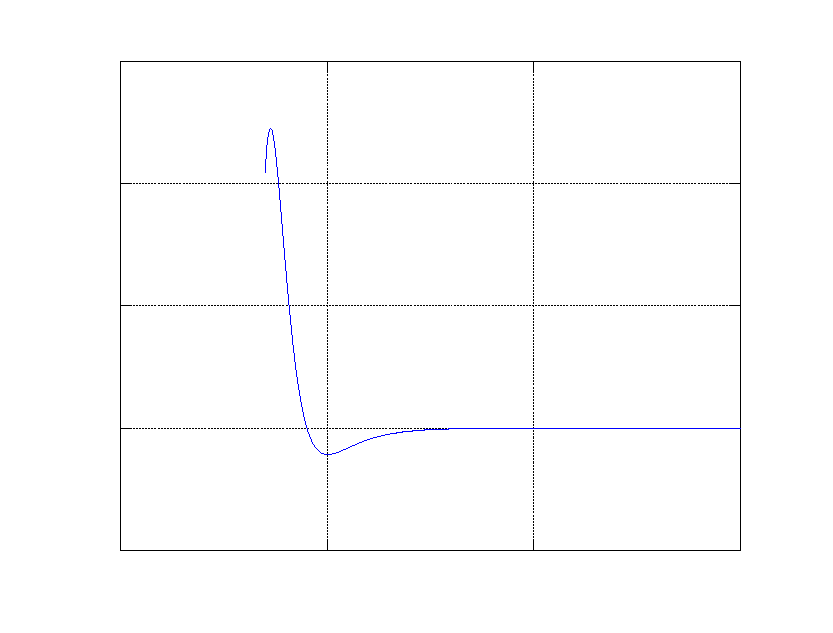
\includegraphics{FormuleQuadratura/analysisFunction517-PlotOutput}}%
    \gplfronttext
  \end{picture}%
\endgroup

\end{center}
Rappresento la derivata seconda (in rosso) e la derivata quarta (in verde),
questo plot utilizza per entrambi gli assi una scala logaritmica:
\begin{center}   
% GNUPLOT: LaTeX picture with Postscript
\begingroup
  \makeatletter
  \providecommand\color[2][]{%
    \GenericError{(gnuplot) \space\space\space\@spaces}{%
      Package color not loaded in conjunction with
      terminal option `colourtext'%
    }{See the gnuplot documentation for explanation.%
    }{Either use 'blacktext' in gnuplot or load the package
      color.sty in LaTeX.}%
    \renewcommand\color[2][]{}%
  }%
  \providecommand\includegraphics[2][]{%
    \GenericError{(gnuplot) \space\space\space\@spaces}{%
      Package graphicx or graphics not loaded%
    }{See the gnuplot documentation for explanation.%
    }{The gnuplot epslatex terminal needs graphicx.sty or graphics.sty.}%
    \renewcommand\includegraphics[2][]{}%
  }%
  \providecommand\rotatebox[2]{#2}%
  \@ifundefined{ifGPcolor}{%
    \newif\ifGPcolor
    \GPcolortrue
  }{}%
  \@ifundefined{ifGPblacktext}{%
    \newif\ifGPblacktext
    \GPblacktexttrue
  }{}%
  % define a \g@addto@macro without @ in the name:
  \let\gplgaddtomacro\g@addto@macro
  % define empty templates for all commands taking text:
  \gdef\gplbacktext{}%
  \gdef\gplfronttext{}%
  \makeatother
  \ifGPblacktext
    % no textcolor at all
    \def\colorrgb#1{}%
    \def\colorgray#1{}%
  \else
    % gray or color?
    \ifGPcolor
      \def\colorrgb#1{\color[rgb]{#1}}%
      \def\colorgray#1{\color[gray]{#1}}%
      \expandafter\def\csname LTw\endcsname{\color{white}}%
      \expandafter\def\csname LTb\endcsname{\color{black}}%
      \expandafter\def\csname LTa\endcsname{\color{black}}%
      \expandafter\def\csname LT0\endcsname{\color[rgb]{1,0,0}}%
      \expandafter\def\csname LT1\endcsname{\color[rgb]{0,1,0}}%
      \expandafter\def\csname LT2\endcsname{\color[rgb]{0,0,1}}%
      \expandafter\def\csname LT3\endcsname{\color[rgb]{1,0,1}}%
      \expandafter\def\csname LT4\endcsname{\color[rgb]{0,1,1}}%
      \expandafter\def\csname LT5\endcsname{\color[rgb]{1,1,0}}%
      \expandafter\def\csname LT6\endcsname{\color[rgb]{0,0,0}}%
      \expandafter\def\csname LT7\endcsname{\color[rgb]{1,0.3,0}}%
      \expandafter\def\csname LT8\endcsname{\color[rgb]{0.5,0.5,0.5}}%
    \else
      % gray
      \def\colorrgb#1{\color{black}}%
      \def\colorgray#1{\color[gray]{#1}}%
      \expandafter\def\csname LTw\endcsname{\color{white}}%
      \expandafter\def\csname LTb\endcsname{\color{black}}%
      \expandafter\def\csname LTa\endcsname{\color{black}}%
      \expandafter\def\csname LT0\endcsname{\color{black}}%
      \expandafter\def\csname LT1\endcsname{\color{black}}%
      \expandafter\def\csname LT2\endcsname{\color{black}}%
      \expandafter\def\csname LT3\endcsname{\color{black}}%
      \expandafter\def\csname LT4\endcsname{\color{black}}%
      \expandafter\def\csname LT5\endcsname{\color{black}}%
      \expandafter\def\csname LT6\endcsname{\color{black}}%
      \expandafter\def\csname LT7\endcsname{\color{black}}%
      \expandafter\def\csname LT8\endcsname{\color{black}}%
    \fi
  \fi
  \setlength{\unitlength}{0.0500bp}%
  \begin{picture}(7680.00,5760.00)%
    \gplgaddtomacro\gplbacktext{%
      \colorrgb{0.00,0.00,0.00}%
      \put(866,633){\makebox(0,0)[r]{\strut{}$10^{-2}$}}%
      \colorrgb{0.00,0.00,0.00}%
      \put(866,1304){\makebox(0,0)[r]{\strut{}$10^{-1}$}}%
      \colorrgb{0.00,0.00,0.00}%
      \put(866,1974){\makebox(0,0)[r]{\strut{}$10^{0}$}}%
      \colorrgb{0.00,0.00,0.00}%
      \put(866,2645){\makebox(0,0)[r]{\strut{}$10^{1}$}}%
      \colorrgb{0.00,0.00,0.00}%
      \put(866,3315){\makebox(0,0)[r]{\strut{}$10^{2}$}}%
      \colorrgb{0.00,0.00,0.00}%
      \put(866,3986){\makebox(0,0)[r]{\strut{}$10^{3}$}}%
      \colorrgb{0.00,0.00,0.00}%
      \put(866,4656){\makebox(0,0)[r]{\strut{}$10^{4}$}}%
      \colorrgb{0.00,0.00,0.00}%
      \put(866,5327){\makebox(0,0)[r]{\strut{}$10^{5}$}}%
      \colorrgb{0.00,0.00,0.00}%
      \put(998,413){\makebox(0,0){\strut{}$10^{-1}$}}%
      \colorrgb{0.00,0.00,0.00}%
      \put(2982,413){\makebox(0,0){\strut{}$10^{0}$}}%
      \colorrgb{0.00,0.00,0.00}%
      \put(4965,413){\makebox(0,0){\strut{}$10^{1}$}}%
      \colorrgb{0.00,0.00,0.00}%
      \put(6949,413){\makebox(0,0){\strut{}$10^{2}$}}%
    }%
    \gplgaddtomacro\gplfronttext{%
    }%
    \gplbacktext
    \put(0,0){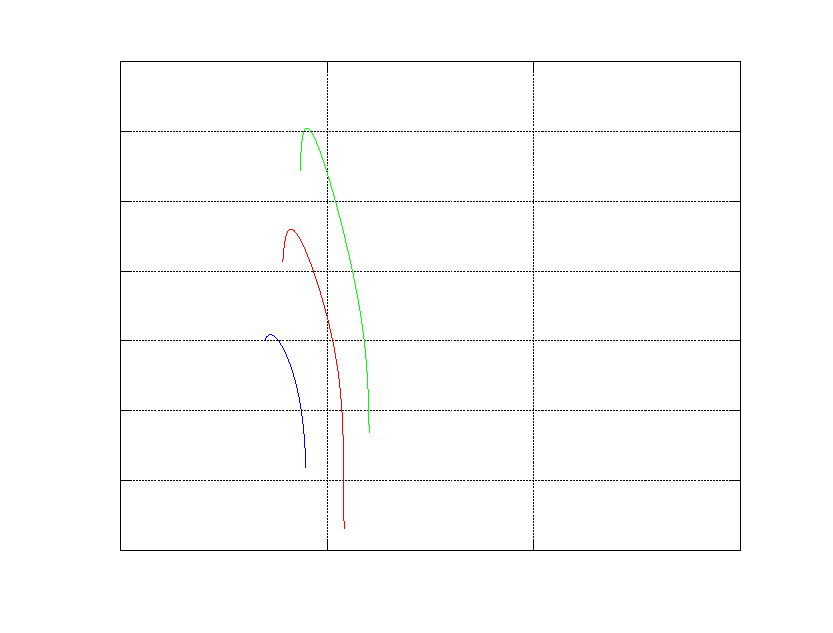
\includegraphics{FormuleQuadratura/analysisFunction517WithDers-PlotOutput}}%
    \gplfronttext
  \end{picture}%
\endgroup

\end{center} 
I precedenti plot si possono ricavare utilizzando il codice
\nameref{subsec:functionPlotter517}.

\begin{exercise}[5.4] 
Per il testo dell'esercizio consultare il libro di testo.
\end{exercise}
Vedere il codice \nameref{subsec:exercise54}.

\begin{exercise}[5.5] 
Per il testo dell'esercizio consultare il libro di testo.
\end{exercise}
Vedere il codice \nameref{subsec:exercise55}.

\begin{exercise}[5.6] 
Per il testo dell'esercizio consultare il libro di testo.
\end{exercise}
Vedere il codice \nameref{subsec:adaptiveTrapezi}.

\begin{exercise}[5.7] 
Per il testo dell'esercizio consultare il libro di testo.
\end{exercise}
Vedere il codice \nameref{subsec:adaptiveSimpson}.

\begin{exercise}[5.9, 5.10 tabelle per schemi compositi] 
Per i testi degli esercizi consultare il libro di testo.
\end{exercise}
Il seguente output \`e generato usando il codice
\nameref{subsec:exercise59solver}.
\begin{lstlisting}
[trapeziCompositeResultTable, simpsonCompositeResultTable] = exercise59solver
trapeziCompositeResultTable =

   1.0000e+03   6.6401e-01  -1.7771e+00
   2.0000e+03   7.3077e-01  -4.4427e-01
   3.0000e+03   7.4507e-01  -1.9745e-01
   4.0000e+03   7.5020e-01  -1.1107e-01
   5.0000e+03   7.5260e-01  -7.1083e-02
   6.0000e+03   7.5391e-01  -4.9363e-02
   7.0000e+03   7.5470e-01  -3.6267e-02
   8.0000e+03   7.5522e-01  -2.7767e-02
   9.0000e+03   7.5557e-01  -2.1939e-02
   1.0000e+04   7.5582e-01  -1.7771e-02

simpsonCompositeResultTable =

   1.0000e+03   7.0132e-01  -1.3618e-01
   2.0000e+03   7.5303e-01  -8.5114e-03
   3.0000e+03   7.5617e-01  -1.6813e-03
   4.0000e+03   7.5668e-01  -5.3196e-04
   5.0000e+03   7.5681e-01  -2.1789e-04
   6.0000e+03   7.5686e-01  -1.0508e-04
   7.0000e+03   7.5688e-01  -5.6719e-05
   8.0000e+03   7.5689e-01  -3.3248e-05
   9.0000e+03   7.5689e-01  -2.0756e-05
   1.0000e+04   7.5690e-01  -1.3618e-05
\end{lstlisting}
nelle precedenti matrici si ha valorizzato nella prima colonna il numero di
sottointervalli, nella seconda \\
l'approssimazione dell'integrale e nella terza l'errore che si commette.

\begin{exercise}[5.9, 5.10 tabelle per schemi adattivi] 
Per i testi degli esercizi consultare il libro di testo.
\end{exercise}
Il seguente output \`e generato usando il codice
\nameref{subsec:exercise510solver}.
\begin{lstlisting}
octave:2> [trapeziAdaptiveResultTable, simpsonAdaptiveResultTable] = exercise510solver
trapeziAdaptiveResultTable =

   1.0000e-01   5.8198e-03   1.5900e+02
   1.0000e-02   1.1881e-03   4.7100e+02
   1.0000e-03   2.9774e-04   1.5670e+03
   1.0000e-04   5.8566e-05   4.8510e+03
   1.0000e-05   5.5259e-06   1.4823e+04

simpsonAdaptiveResultTable =

   1.0000e-01   5.4037e-04   4.9000e+01
   1.0000e-02   2.1963e-04   6.5000e+01
   1.0000e-03   4.8899e-05   9.3000e+01
   1.0000e-04   1.2482e-05   1.8100e+02
   1.0000e-05   3.3642e-06   3.0900e+02
\end{lstlisting}
nelle precedenti matrici si ha valorizzato nella prima colonna la tollerenza
richiesta, nella seconda l'errore che si commette e nella terza il numero di
punti necessari per raggiungere la precisione richiesta.

Rappresento i punti sulla funzione integranda utilizzati dal metodo adattivo di
Simpson per raggiungere una precisione di $10^{-4}$:
\begin{center}   
% GNUPLOT: LaTeX picture with Postscript
\begingroup
  \makeatletter
  \providecommand\color[2][]{%
    \GenericError{(gnuplot) \space\space\space\@spaces}{%
      Package color not loaded in conjunction with
      terminal option `colourtext'%
    }{See the gnuplot documentation for explanation.%
    }{Either use 'blacktext' in gnuplot or load the package
      color.sty in LaTeX.}%
    \renewcommand\color[2][]{}%
  }%
  \providecommand\includegraphics[2][]{%
    \GenericError{(gnuplot) \space\space\space\@spaces}{%
      Package graphicx or graphics not loaded%
    }{See the gnuplot documentation for explanation.%
    }{The gnuplot epslatex terminal needs graphicx.sty or graphics.sty.}%
    \renewcommand\includegraphics[2][]{}%
  }%
  \providecommand\rotatebox[2]{#2}%
  \@ifundefined{ifGPcolor}{%
    \newif\ifGPcolor
    \GPcolortrue
  }{}%
  \@ifundefined{ifGPblacktext}{%
    \newif\ifGPblacktext
    \GPblacktexttrue
  }{}%
  % define a \g@addto@macro without @ in the name:
  \let\gplgaddtomacro\g@addto@macro
  % define empty templates for all commands taking text:
  \gdef\gplbacktext{}%
  \gdef\gplfronttext{}%
  \makeatother
  \ifGPblacktext
    % no textcolor at all
    \def\colorrgb#1{}%
    \def\colorgray#1{}%
  \else
    % gray or color?
    \ifGPcolor
      \def\colorrgb#1{\color[rgb]{#1}}%
      \def\colorgray#1{\color[gray]{#1}}%
      \expandafter\def\csname LTw\endcsname{\color{white}}%
      \expandafter\def\csname LTb\endcsname{\color{black}}%
      \expandafter\def\csname LTa\endcsname{\color{black}}%
      \expandafter\def\csname LT0\endcsname{\color[rgb]{1,0,0}}%
      \expandafter\def\csname LT1\endcsname{\color[rgb]{0,1,0}}%
      \expandafter\def\csname LT2\endcsname{\color[rgb]{0,0,1}}%
      \expandafter\def\csname LT3\endcsname{\color[rgb]{1,0,1}}%
      \expandafter\def\csname LT4\endcsname{\color[rgb]{0,1,1}}%
      \expandafter\def\csname LT5\endcsname{\color[rgb]{1,1,0}}%
      \expandafter\def\csname LT6\endcsname{\color[rgb]{0,0,0}}%
      \expandafter\def\csname LT7\endcsname{\color[rgb]{1,0.3,0}}%
      \expandafter\def\csname LT8\endcsname{\color[rgb]{0.5,0.5,0.5}}%
    \else
      % gray
      \def\colorrgb#1{\color{black}}%
      \def\colorgray#1{\color[gray]{#1}}%
      \expandafter\def\csname LTw\endcsname{\color{white}}%
      \expandafter\def\csname LTb\endcsname{\color{black}}%
      \expandafter\def\csname LTa\endcsname{\color{black}}%
      \expandafter\def\csname LT0\endcsname{\color{black}}%
      \expandafter\def\csname LT1\endcsname{\color{black}}%
      \expandafter\def\csname LT2\endcsname{\color{black}}%
      \expandafter\def\csname LT3\endcsname{\color{black}}%
      \expandafter\def\csname LT4\endcsname{\color{black}}%
      \expandafter\def\csname LT5\endcsname{\color{black}}%
      \expandafter\def\csname LT6\endcsname{\color{black}}%
      \expandafter\def\csname LT7\endcsname{\color{black}}%
      \expandafter\def\csname LT8\endcsname{\color{black}}%
    \fi
  \fi
  \setlength{\unitlength}{0.0500bp}%
  \begin{picture}(7680.00,5760.00)%
    \gplgaddtomacro\gplbacktext{%
      \colorrgb{0.00,0.00,0.00}%
      \put(866,633){\makebox(0,0)[r]{\strut{}-5}}%
      \colorrgb{0.00,0.00,0.00}%
      \put(866,1807){\makebox(0,0)[r]{\strut{}0}}%
      \colorrgb{0.00,0.00,0.00}%
      \put(866,2980){\makebox(0,0)[r]{\strut{}5}}%
      \colorrgb{0.00,0.00,0.00}%
      \put(866,4154){\makebox(0,0)[r]{\strut{}10}}%
      \colorrgb{0.00,0.00,0.00}%
      \put(866,5327){\makebox(0,0)[r]{\strut{}15}}%
      \colorrgb{0.00,0.00,0.00}%
      \put(998,413){\makebox(0,0){\strut{}$10^{-1}$}}%
      \colorrgb{0.00,0.00,0.00}%
      \put(2982,413){\makebox(0,0){\strut{}$10^{0}$}}%
      \colorrgb{0.00,0.00,0.00}%
      \put(4965,413){\makebox(0,0){\strut{}$10^{1}$}}%
      \colorrgb{0.00,0.00,0.00}%
      \put(6949,413){\makebox(0,0){\strut{}$10^{2}$}}%
    }%
    \gplgaddtomacro\gplfronttext{%
    }%
    \gplbacktext
    \put(0,0){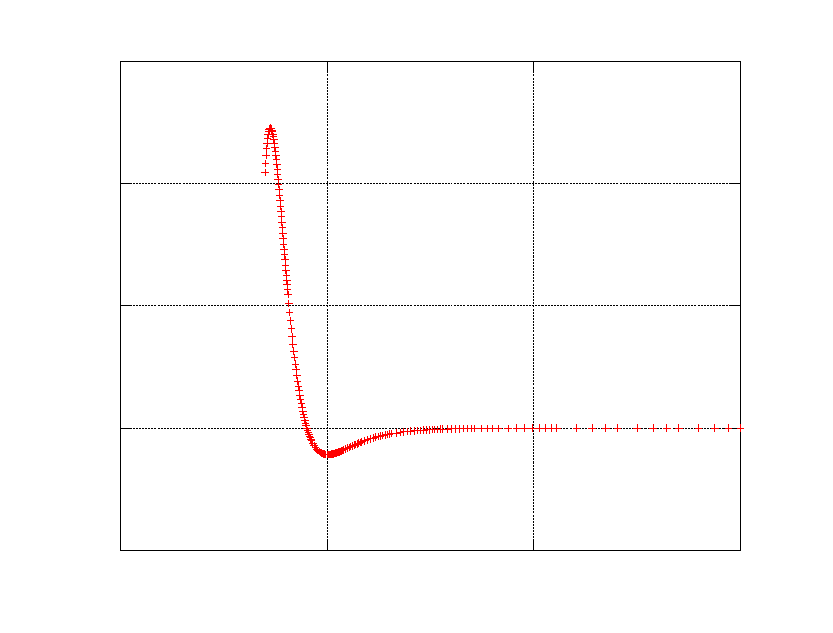
\includegraphics{FormuleQuadratura/exercise510-SimpsonAdaptivePlotOutput}}%
    \gplfronttext
  \end{picture}%
\endgroup

\end{center}

Rappresento i punti sulla funzione integranda utilizzati dal metodo adattivo dei
Trapezi per raggiungere una precisione di $10^{-3}$:
\begin{center}   
% GNUPLOT: LaTeX picture with Postscript
\begingroup
  \makeatletter
  \providecommand\color[2][]{%
    \GenericError{(gnuplot) \space\space\space\@spaces}{%
      Package color not loaded in conjunction with
      terminal option `colourtext'%
    }{See the gnuplot documentation for explanation.%
    }{Either use 'blacktext' in gnuplot or load the package
      color.sty in LaTeX.}%
    \renewcommand\color[2][]{}%
  }%
  \providecommand\includegraphics[2][]{%
    \GenericError{(gnuplot) \space\space\space\@spaces}{%
      Package graphicx or graphics not loaded%
    }{See the gnuplot documentation for explanation.%
    }{The gnuplot epslatex terminal needs graphicx.sty or graphics.sty.}%
    \renewcommand\includegraphics[2][]{}%
  }%
  \providecommand\rotatebox[2]{#2}%
  \@ifundefined{ifGPcolor}{%
    \newif\ifGPcolor
    \GPcolortrue
  }{}%
  \@ifundefined{ifGPblacktext}{%
    \newif\ifGPblacktext
    \GPblacktexttrue
  }{}%
  % define a \g@addto@macro without @ in the name:
  \let\gplgaddtomacro\g@addto@macro
  % define empty templates for all commands taking text:
  \gdef\gplbacktext{}%
  \gdef\gplfronttext{}%
  \makeatother
  \ifGPblacktext
    % no textcolor at all
    \def\colorrgb#1{}%
    \def\colorgray#1{}%
  \else
    % gray or color?
    \ifGPcolor
      \def\colorrgb#1{\color[rgb]{#1}}%
      \def\colorgray#1{\color[gray]{#1}}%
      \expandafter\def\csname LTw\endcsname{\color{white}}%
      \expandafter\def\csname LTb\endcsname{\color{black}}%
      \expandafter\def\csname LTa\endcsname{\color{black}}%
      \expandafter\def\csname LT0\endcsname{\color[rgb]{1,0,0}}%
      \expandafter\def\csname LT1\endcsname{\color[rgb]{0,1,0}}%
      \expandafter\def\csname LT2\endcsname{\color[rgb]{0,0,1}}%
      \expandafter\def\csname LT3\endcsname{\color[rgb]{1,0,1}}%
      \expandafter\def\csname LT4\endcsname{\color[rgb]{0,1,1}}%
      \expandafter\def\csname LT5\endcsname{\color[rgb]{1,1,0}}%
      \expandafter\def\csname LT6\endcsname{\color[rgb]{0,0,0}}%
      \expandafter\def\csname LT7\endcsname{\color[rgb]{1,0.3,0}}%
      \expandafter\def\csname LT8\endcsname{\color[rgb]{0.5,0.5,0.5}}%
    \else
      % gray
      \def\colorrgb#1{\color{black}}%
      \def\colorgray#1{\color[gray]{#1}}%
      \expandafter\def\csname LTw\endcsname{\color{white}}%
      \expandafter\def\csname LTb\endcsname{\color{black}}%
      \expandafter\def\csname LTa\endcsname{\color{black}}%
      \expandafter\def\csname LT0\endcsname{\color{black}}%
      \expandafter\def\csname LT1\endcsname{\color{black}}%
      \expandafter\def\csname LT2\endcsname{\color{black}}%
      \expandafter\def\csname LT3\endcsname{\color{black}}%
      \expandafter\def\csname LT4\endcsname{\color{black}}%
      \expandafter\def\csname LT5\endcsname{\color{black}}%
      \expandafter\def\csname LT6\endcsname{\color{black}}%
      \expandafter\def\csname LT7\endcsname{\color{black}}%
      \expandafter\def\csname LT8\endcsname{\color{black}}%
    \fi
  \fi
  \setlength{\unitlength}{0.0500bp}%
  \begin{picture}(7680.00,5760.00)%
    \gplgaddtomacro\gplbacktext{%
      \colorrgb{0.00,0.00,0.00}%
      \put(866,633){\makebox(0,0)[r]{\strut{}-5}}%
      \colorrgb{0.00,0.00,0.00}%
      \put(866,1807){\makebox(0,0)[r]{\strut{}0}}%
      \colorrgb{0.00,0.00,0.00}%
      \put(866,2980){\makebox(0,0)[r]{\strut{}5}}%
      \colorrgb{0.00,0.00,0.00}%
      \put(866,4154){\makebox(0,0)[r]{\strut{}10}}%
      \colorrgb{0.00,0.00,0.00}%
      \put(866,5327){\makebox(0,0)[r]{\strut{}15}}%
      \colorrgb{0.00,0.00,0.00}%
      \put(998,413){\makebox(0,0){\strut{}$10^{-1}$}}%
      \colorrgb{0.00,0.00,0.00}%
      \put(2982,413){\makebox(0,0){\strut{}$10^{0}$}}%
      \colorrgb{0.00,0.00,0.00}%
      \put(4965,413){\makebox(0,0){\strut{}$10^{1}$}}%
      \colorrgb{0.00,0.00,0.00}%
      \put(6949,413){\makebox(0,0){\strut{}$10^{2}$}}%
    }%
    \gplgaddtomacro\gplfronttext{%
    }%
    \gplbacktext
    \put(0,0){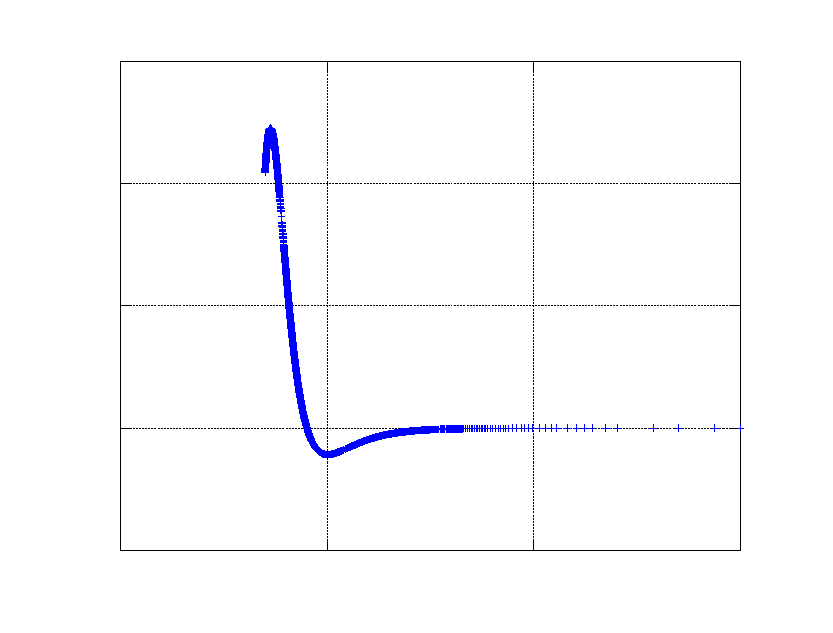
\includegraphics{FormuleQuadratura/exercise510-TrapeziAdaptivePlotOutput}}%
    \gplfronttext
  \end{picture}%
\endgroup

\end{center}
